\documentclass{hertieteaching}
\usepackage{pifont}
\usepackage{relsize}

\title{Text as Data as Measurement}

\begin{document}

\maketitle

% model structure choices
% preprocessing
% strategic considerations

\begin{frame}{Last week}

Last week we talked rather abstractly about models that connected the `message' $\theta$ and the words $W$ (or whatever features we decided to treat as exchangeable)

Let's be a bit more specific

\end{frame}


\begin{frame}{Decisions, decisions}

Are we modeling 
\begin{itemize}
  \item the generation process
  \item the understanding process
  \item or maybe both\ldots
\end{itemize}

\pause

Por qué no los dos?
\begin{align*}
P(\theta) && \textit{Prior expectations}\\
P(\{W\} \mid \theta) && \textit{Generation} \\
P(\theta \mid \{W\}) & = \frac{P(\{W\} \mid \theta)P(\theta)}{\int P(\{W\} \mid \theta) P(\theta) d\theta} & \textit{Understanding}
\end{align*}

\end{frame}
\begin{frame}{Decisions, decisions}
Examples:

Document classification: $\theta$ is the probability that this document is about social policy
\begin{itemize}
  \item Naive Bayes Classification, learn all the things
  \item (Regularized) Logistic Regression, go straight for $P(\theta \mid \{W\})$ 
\end{itemize}

Thematic analysis: $\theta$ is the proportion of social policy mentions in the document
\begin{itemize}
  \item Topic Models, learn all the things
  \item Content Analysis Dictionaries, assert $P(\{W\} \mid \theta)$ and go straight for $P(\theta \mid \{W\})$
\end{itemize}

We'll take a closer look at thematic analysis next week, so let's look at classification

\end{frame}
\begin{frame}{Example}

Example application: \textcite{Evans.etal2007} attempt to 
\begin{itemize}
  \item Distinguish the amicus briefs from each side of two  affirmative action cases: Regents of the University of California v. Bakke (1978) and Grutter/Gratz v. Bollinger 2003. 
  \item Characterize the language used by each side
\end{itemize}
We can label the Plaintiff as `Conservative' and the Respondents as `Liberal'

\medskip
\begin{quote}
All told, Bakke included 57 amicus briefs (15 for the conservative
side and 42 for liberals) and Bollinger received 93 (19
conservative and 74 liberal).\\
\hfill\parencite{Evans.etal2007}
\end{quote}

The four briefs of Plaintiffs and Respondents formed the `training data`

\end{frame}
\begin{frame}{Naive Bayes Classification}

The document category is $Z \in \{\text{Lib}, \text{Con}\}$ 
\begin{align*}
P(Z) & = \theta & \textit{Prior probability}\\
P(\{W\} \mid Z) & = \prod_j P(W_j \mid Z) & \textit{The naive part}
\end{align*}
Words are assumed to be generated 
\textit{independently} given the category Z
\begin{align*}
P( \text{`Affirmative Action'} \mid Z=\text{`Lib'}) &~=~ P( \text{`Affirmative'} \mid Z=\text{`Lib'}) 
 P( \text{`Action'} \mid Z=\text{`Lib'})
\end{align*}
\pause
Classification here means doing something with 
$$
P(Z \mid \{W\})
$$
the \textit{posterior distribution}
\begin{itemize}
  \item Strictly, this is just probability estimation.  Classification is a separate decision problem.
\end{itemize}


\end{frame}



\begin{frame}[t,fragile]\frametitle{Naive Bayes}

Estimating $\theta = P(Z = \text{Lib}) = (1 - P(Z = \text{Con}))$ is easy. 
\begin{itemize}
  \item Count the Liberal documents and divide by the total number of documents
\end{itemize}

Similarly, estimating $P(W_v \mid X)$ is straightforward
$$
P(W_j \mid Z = \text{`Lib'}) = \frac{C_j}{\sum^{W \in \text{`Lib'}}_v C_v}
$$
where $C_v$ is the count of tokens of $W_v$.

Actually at this point we have a modeling choice \parencite{McCallum.Nigam1993}:
\begin{itemize}
  \item $P(W_j \mid Z = \text{Lib})$ is Binomial
  \item $P([W_1 \ldots W_V] \mid Z = \text{Lib})$ is Multinomial
  \item Some \textit{transformation} of $P([W_1 \ldots W_V] \mid Z = \text{Lib})$ (e.g. `tfidf') is Normal
\end{itemize}

\end{frame}
\begin{frame}[t,fragile]\frametitle{Naive Bayes}


%The classifier then chooses the class Z (Liberal or Conservative) with the highest aggregate probability.

Every new word adds a bit of information that re-adjusts the conditional probabilities.

\begin{align*}
\frac{P(Z=\text{{`Lib'}} \mid \{W\})}
{P(Z=\text{`Con'} \mid \{W\})} & ~=~ 
\mathlarger{\prod} \frac{P(W_j \mid Z=\text{\text{`Lib'}})}
{P(W_j \mid Z=\text{`Con'})}\times \frac{P(Z=\text{\text{`Lib'}})}{~P(Z=\text{`Con'})}
\end{align*}



\end{frame}
%\begin{frame}[t,fragile]\frametitle{Naive Bayes}


%%%%%%%%%%% check the below works in the real document

%[will@Apparent lib]$ ykcats -dictionary ../../disc.vbpro ../lib/*
%,Dictionary,Dictionary>discrimination,WordCount
%6019_ll01-utf8.txt,26,26,20002
%6020_ll01-utf8.txt,13,13,18722
%[will@Apparent lib]$ ykcats -dictionary ../../disc.vbpro ../con/*
%,Dictionary,Dictionary>discrimination,WordCount
%6019_lc01-utf8.txt,70,70,17368
%6020_lc01-utf8.txt,48,48,17698

% lib = (26+13)/(20002+18722) = 0.001007127
% con = (70+48)/(17368+17698) = 0.003365083
% lib / con = .299

%%%%%%%%%%%

%\end{frame}
\begin{frame}[t,fragile]\frametitle{Discrimination}

Example: Naive Bayes with only word class `discriminat*'.

Assume that liberal and conservative supporting briefs are equally likely (true in the training set)
\begin{align*}
\frac{P(Z=\text{\text{`Lib'}})}{P(Z=\text{`Con'})} & = 1
\end{align*}
and
\begin{align*}
P(W=\text{`discriminat*'} \mid Z=\text{`Lib'}) & = (26+13)/(20002+18722) \approx 0.001\\
P(W=\text{`discriminat*'} \mid Z=\text{`Con'}) & = (70+48)/(17368+17698) \approx 0.003
\end{align*}

Posterior probability ratio is about 1/3 in favour of the document supporting the conservative side

\end{frame}

\begin{frame}\frametitle{Conservative vocabulary}
\centerline{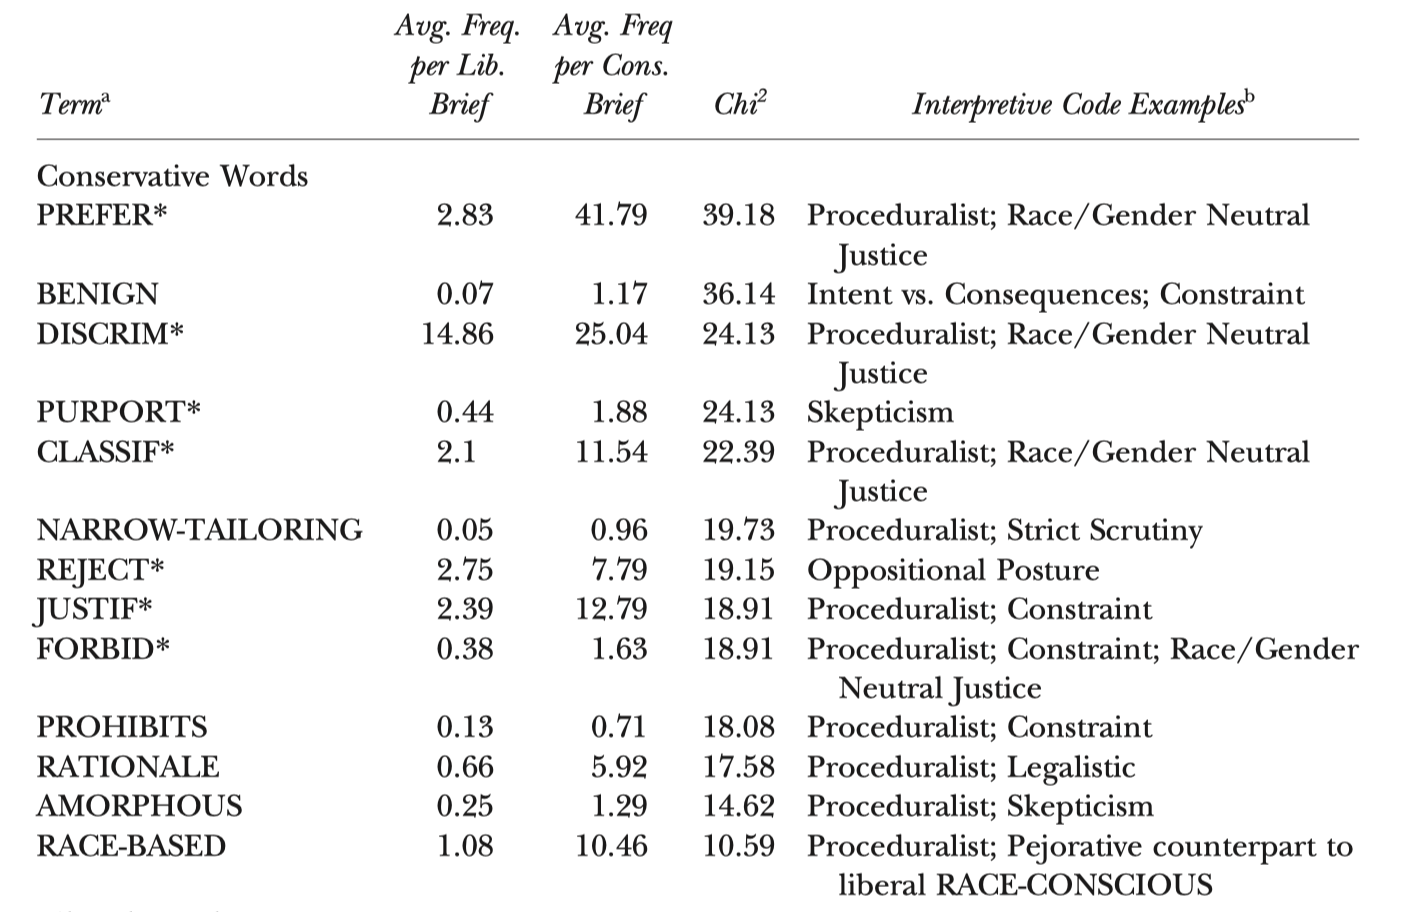
\includegraphics[scale=0.4]{pictures/evansetal1.png}}
\end{frame}

\begin{frame}\frametitle{Liberal vocabulary}

\medskip
\centerline{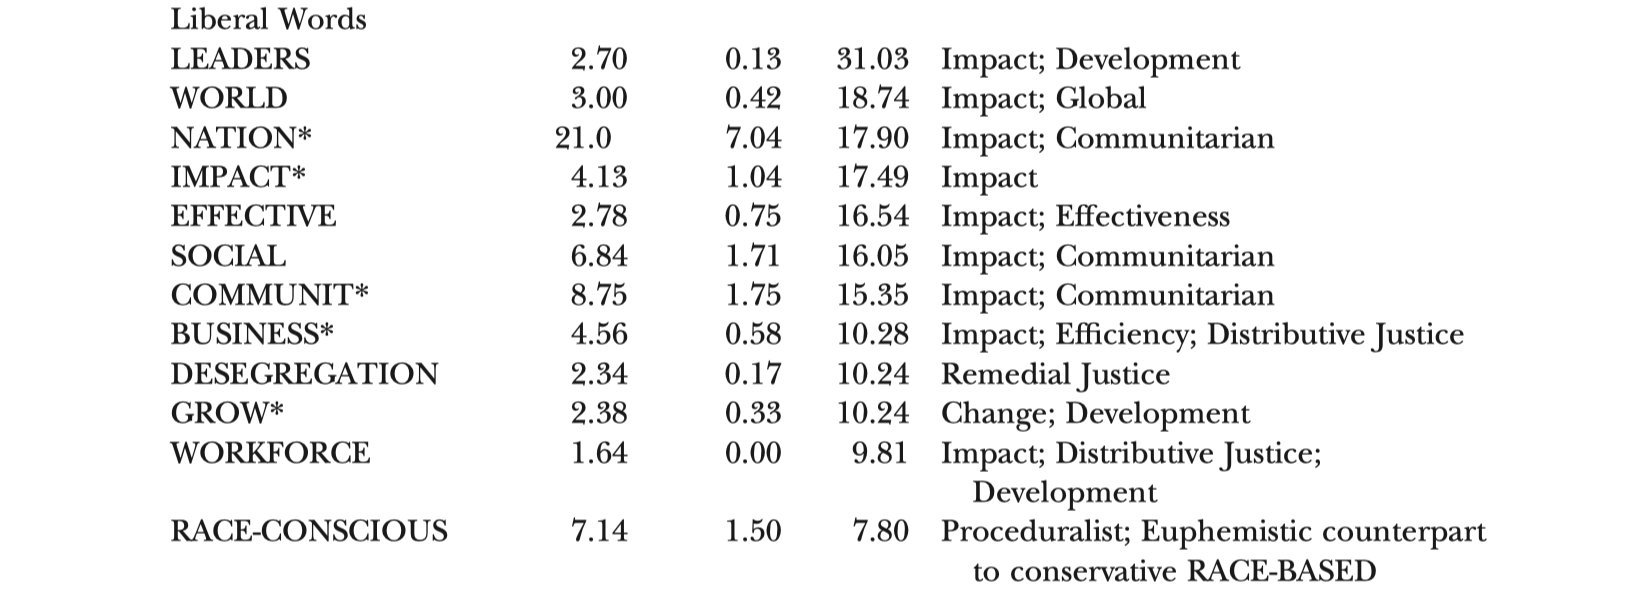
\includegraphics[scale=0.4]{pictures/evansetal2.png}}

\begin{itemize}
  \item There are no identifiable \textit{uniquely} partisan words  
  \item but these associations are stable in cases 28 years apart
\end{itemize}

\end{frame}

\begin{frame}[t,fragile]\frametitle{Discrimination}

%(File 6019\_al18-utf8.txt)
Amicus brief from `King County Bar Association' containing 3667 words and 4 matches to disciminat*.

\small
\begin{verbatim}
      that "the state shall not [discriminate] against, or grant preferential treatment
the lingering effects of racial [discrimination] against minority groups in this
 remedy the effects of societal [discrimination]. Another four Justices (Stevens
      that "the state shall not [discriminate] against, or grant preferential treatment
\end{verbatim}
\normalsize

\end{frame}


\begin{frame}[t,fragile]\frametitle{Every generative model}

Courtesy of Bayes theorem, the posterior probability of a document being liberal is
\begin{align*}
P(Z = \text{`Lib'} \mid W_j) & = \frac{\prod P(W_j \mid Z = \text{`Lib'}) P(Z = \text{`Lib'})}
{\prod P(W_j \mid Z = \text{`Lib'}) P(Z = \text{`Lib'}) + \prod P(W_j \mid Z = \text{`Con'}) P(Z = \text{`Con'})}
\intertext{but let's do a little rearranging}
P(Z = \text{Lib} \mid W_j) & = 
\frac{1}{1 + \text{exp}(-\eta)}\\
\eta &= \log \frac{P(Z = \text{`Lib'})}{P(Z = \text{`Con'})} + 
  \sum_j \log \frac{P(W_j \mid Z = \text{`Lib'})}{P(W_j \mid Z = \text{`Con'})}
\end{align*}
which might remind you of a model you've seen before\ldots

\end{frame}
\begin{frame}[t,fragile]\frametitle{has a discriminative alter ego}

\begin{align*}
P(Z = \text{`Lib'} \mid W_j) & = 
\frac{1}{1 + \text{exp}(-\eta)}\\
\eta &= \beta_0 + C_1 \beta_1 + C_2 \beta_2 + \ldots + C_2 \beta_V
\end{align*}
where $C_v$ is the count of word $v$.


\pause

This is a logistic regression \parencite{Nigam.etal1999}. It's called `MaxEnt' by computational linguists. 

From which we conclude \parencite{Jordan1999}
\begin{itemize}
  \item These are in a certain sense the `same model'
  \item As it happens, \textit{any} exponential family choice for $P(W_j \mid Z)$ has logistic regression as its discriminative model 
\end{itemize}


\end{frame}

\begin{frame}[t,fragile]\frametitle{Naive Bayes and Logit}

Logistic regression is more focused
\begin{itemize}
  \item No interest in $P([W_1 \ldots W_V])$. Words can be conditionally independent, or not. It just wants the decision boundary
\end{itemize}
Slower and hungrier
\begin{itemize}
  \item $\beta$ estimates converge at rate $N$, compared to $\log N$ for Naive Bayes' probability ratios
  \item We fit Naive Bayes on four documents. Logistic regression will require \textit{heavy regularization} to work with so many fewer documents than words
\end{itemize}
Usually better
\begin{itemize}
  \item Classification performance is usually better: lower bias, higher variance
  \item (Interpretation is trickier)
\end{itemize}

\end{frame}

\begin{frame}[t,fragile]\frametitle{The model tradeoff}

This performance tradeoff is very general:
\begin{itemize}
  \item By adding bias (strong assumptions about the data) we can reduce variance
  \item By adding flexibility we can reduce bias and have a more expressive model, but we'll need more and better data
\end{itemize}

The interpretation tradeoff is also general:
\begin{itemize}
  \item Better statistical performance often leads to less interpretable models \parencite{Chang.etal2009}
  \item In social science applications we usually prefer the interpretable side!
\end{itemize}





\end{frame}

\begin{frame}[allowframebreaks]
\frametitle{References}
\printbibliography	
\end{frame}


\end{document}
